
\documentclass[]{article}

\usepackage[]{graphicx}   % para manejar graficos

\usepackage[space]{grffile} % para manejar graficos

\usepackage{caption}

\usepackage{enumerate}    % para hacer listas numeradas

\usepackage{amsmath}        % no se..

\usepackage{amsfonts}     % no se..

\usepackage{authblk}    % para definir las afiliaciones de cada autor

\usepackage{layout}     % no se..


\usepackage[sorting=none]{biblatex}  % para manejar la bibliografia / referencias

\usepackage{lipsum}     % para generar texto random

\usepackage{multicol}   % para usar dos columnas

\usepackage{palatino}   % para que la fuente sea palatino

\usepackage[utf8]{inputenc} % para poder usar tildes

\usepackage[spanish]{babel} % para escribir en español



\addto\captionsspanish{
\def\tablename{Tabla}
}

\usepackage[sc,big,raggedright,bf]{titlesec} % para definir el formato del
%                                              header de cada seccion.

\usepackage[font=small]{caption} % para que la fuente de un epigrafe no tenga el
%                                  mismo tamaño que el cuerpo del texto

\usepackage{geometry}
 \geometry{
 a4paper,
 textwidth={17cm},
 textheight={23cm},
 left={2cm},
 top={2.5cm},
 }

\setlength{\columnsep}{1cm} % para que la separacion entre columnas sea de 1 cm

\graphicspath {{imagenes/}}

\defbibheading{bibliography}{\section{\refname}} % para que bibtex no imponga su
 % header cuando uso \printbibliography, y que se use el de babel

\addbibresource{bibliografia.bib} % para importar el archivo .bib

\title{\textbf{\LARGE{\textsf{MEDICIÓN DE RESPUESTA EN FRECUENCIA Y
 SENSIBILIDAD DE VARIOS MICRÓFONOS}}}}
 % defino el titulo del Paper

\date{} % lo pongo vacio para que no aparezca abajo del abstract

\usepackage{fancyhdr}

%%%%%%%%%%%%%%%%%%%%%%%%%%%%%%%%%%%%%%%%%%%%%%%%%%%%%%%%%%%%%%%%%%%%%%%%%%%%%%%%
% http://www-h.eng.cam.ac.uk/help/tpl/textprocessing/multicol_hint.html
\makeatletter           % esto lo uso para poder definir figuras
\newenvironment{tablehere}    % esto lo uso para poder definir figuras
  {\def\@captype{table}}    % esto lo uso para poder definir figuras

  {}              % esto lo uso para poder definir figuras
                  % esto lo uso para poder definir figuras
\newenvironment{figurehere}   % esto lo uso para poder definir figuras
  {\def\@captype{figure}}   % esto lo uso para poder definir figuras
  {\par\medskip}
  {}              % esto lo uso para poder definir figuras
\makeatother          % esto lo uso para poder definir figuras
%%%%%%%%%%%%%%%%%%%%%%%%%%%%%%%%%%%%%%%%%%%%%%%%%%%%%%%%%%%%%%%%%%%%%%%%%%%%%%%%

%%%%%%%%%%%%%%%%%%%%%%%%%%%%%%%%%%%%%%%%%%%%%%%%%%%%%%%%%%%%%%%%%%%%%%%%%%%%%%%%
%               ACA EMPIEZA EL DOCUMENTO                            %
%%%%%%%%%%%%%%%%%%%%%%%%%%%%%%%%%%%%%%%%%%%%%%%%%%%%%%%%%%%%%%%%%%%%%%%%%%%%%%%%


\begin{document} % empieza el documentoo


\renewcommand{\headrulewidth}{0pt} % para que no haya linea decorativa en el header.


\author[1]{Federico Feldsberg} % defino el autor
\affil[1]{Universidad Nacional de Tres De Febrero, Buenos Aires, Argentina \newline \texttt{fedefelds@hotmail.com}} % afiliacion del autor


\begin{minipage}[h]{\textwidth} % uso el entorno minipage para que el abstract este en la misma pagina que el titulo
    \maketitle
    \thispagestyle{fancy}
    \fancyhf{}
    \rhead{\today}
    \lhead{Electroacústica I}
    \cfoot{\thepage}

\end{minipage}


\begin{abstract}
\textit{En este artículo se describe una serie de mediciones llevadas a cabo
en el marco de la materia Electroacústica I. Se recurre a dos métodos
de medición distintos para caracterizar los micrófonos Shure SM57,
Rode NT2000, Earthworks M50 y Beyerdynamic MM1.}
\end{abstract}

\begin{multicols}{2}
\section{Introducción}
El presente trabajo tiene como objetivo describir los procesos de medición
llevados a cabo en el marco de la materia Electroacústica I, así como analizar
los resultados allí obtenidos desde el marco teórico de la misma.

Las mediciones están relacionadas con los conceptos de sensibilidad y respuesta
 en frecuencia de micrófonos. Se consideran dos micrófonos durante todo el
proceso: uno se utiliza como micrófono referencia, y el micrófono a medir, de
sensibilidad y respuesta en frecuencia desconocidas. Se utilizaron dos métodos
de medición: el método clásico de Davis y otro método moderno basado en la
función de transferencia.
\section{Método clásico}
El método clásico propuesto por Davis en \cite{davis} permite medir
la sensibilidad y la respuesta en frecuencia de un micrófono dado.

Para este método se utiliza el siguiente instrumental:
\begin{itemize}
\item una consola mezcladora Behringer
\item un parlante de monitoreo KRK
\item un sonómetro Svantek y su calibrador
\item un multímetro digital Uni-T
\item un osciloscopio digital Tektronix
\item un micrófono de referencia Earthworks M50
\end{itemize}

\subsection{Medición de sensibilidad}
En primer lugar, se mide el piso de ruido en el lugar de medición para asegurarse
de que el mismo no afecte las demás mediciones. Se calibra el sonómetro con el
tono puro de 1 kHz que emite su calibrador, de manera que este último detecte un
nivel de presión sonora de referencia de 94 dBSPL, y calcule las compensaciones
necesarias. Ademas se le asigna un tiempo de integración lento.

Dicho método consiste en utilizar un micrófono de referencia, cuya sensibilidad
es conocida. El micrófono de referencia utilizado es el Earthworks M50
Debido a su respuesta en frecuencia prácticamente plana, es considerado un
micrófono ideal o de referencia. Tanto el micrófono de referencia como el
micrófono a medir se colocan a una distancia de 15 cm del parlante para poder
asegurar el nivel de presión sonora deseado.

La figura \ref{fig:bloque_clasico} indica el arreglo instrumental utilizado en el
método clásico

\begin{figurehere}
 \centering
 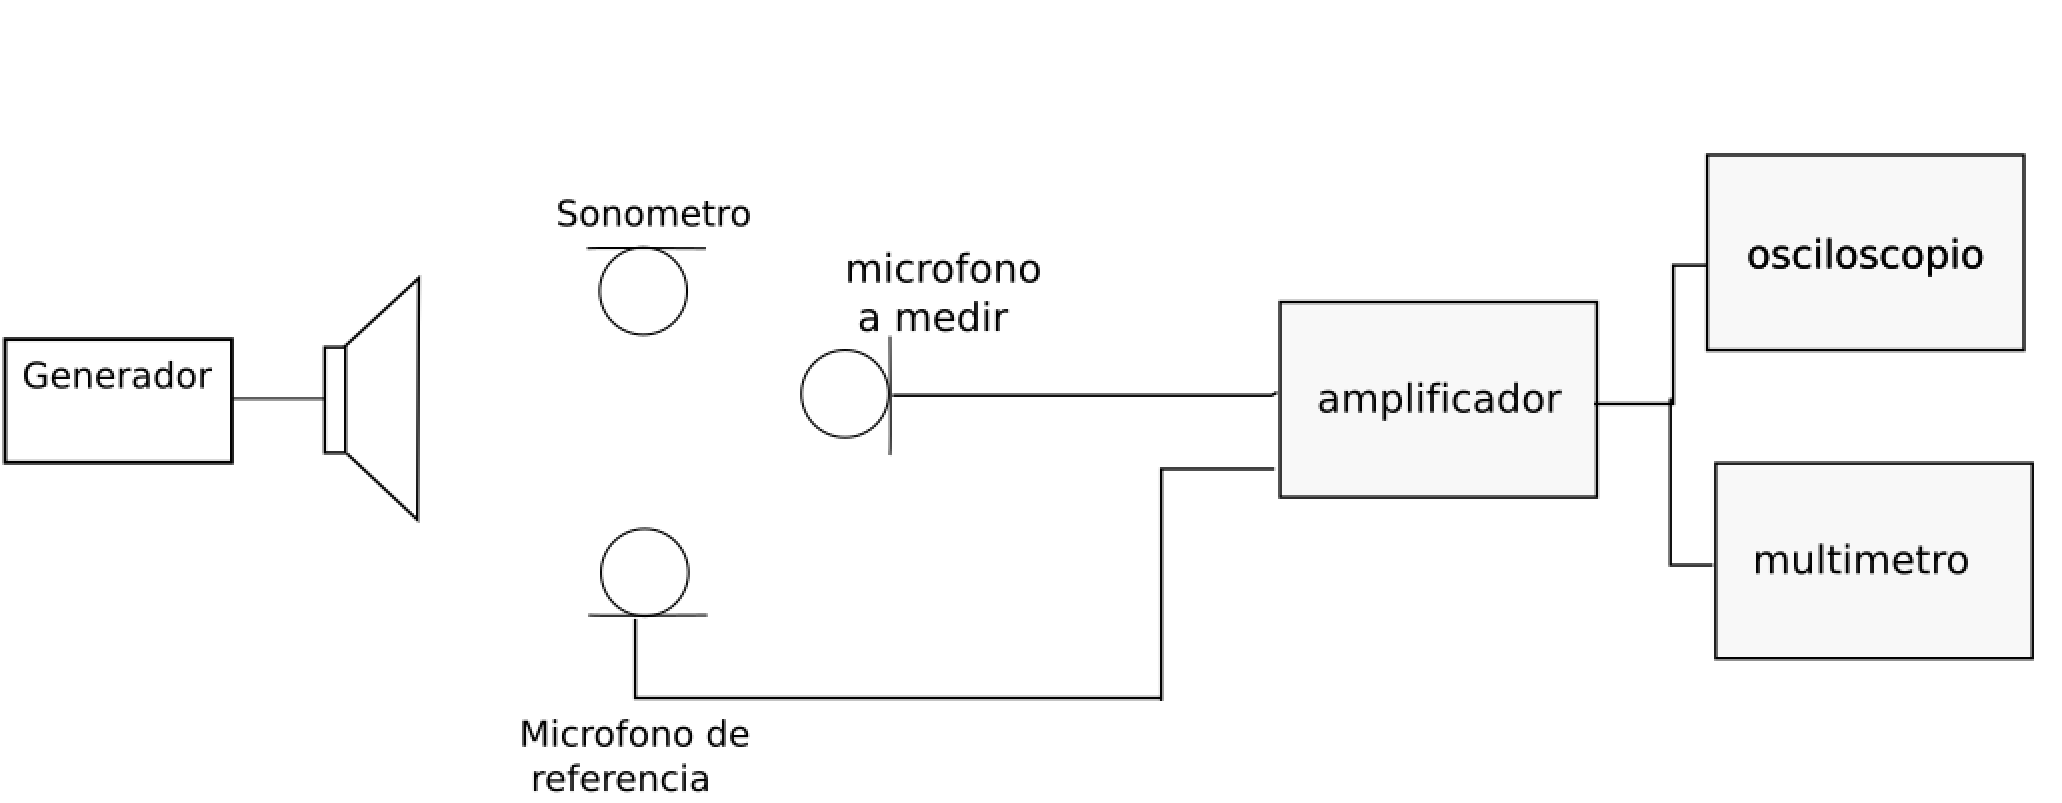
\includegraphics[width=\linewidth]{blockdiag}
 \captionof{figure}{Arreglo instrumental del método clásico}
 \label{fig:bloque_clasico}
\end{figurehere}

El micrófono de referencia es expuesto a un tono puro de 1 kHz a un nivel de
presión sonora de 94 dB SPL. El nivel de presión sonora es controlado con el
sonómeto Svantek. Debido a que no poseemos instrumental lo suficientemente
preciso para medir tensiones en el orden de magnitud de los mV, debemos amplificar
la tensión generada en los terminales del micrófono mediante el uso de una
consola mezcladora. La forma de onda de la salida de dicha consola es monitoreada
por medio de un osciloscopio digital, a modo de hallar una ganancia tal que la
salida de la consola sea medible por nuestro instrumental y
aun así no ocasione recortes de señal. Dicha ganancia se fija para toda la medición.

La sensibilidad de un micrófono $S_0$ esta definida como la tensión en los terminales
de salida del mismo, al estar expuesto a un nivel de presión sonora de 94 dB SPL.
Debido a que la sensibilidad de nuestro micrófono de referencia es conocida,
podemos averiguar la ganancia de la consola si consideramos las ecuaciones
\ref{eq:veces} y \ref{eq:dB}.

\begin{equation}
  G_v=\frac{V_o}{V_i}
  \label{eq:veces}
\end{equation}

\begin{equation}
  G_{dB}= 20 \log \left(\frac{V_o}{V_i}\right)
  \label{eq:dB}
\end{equation}

Bajo las condiciones de esta medición $V_o$ es conocido y $V_i$=$S_0$, por lo que
la ganancia de la consola queda determinada tanto en veces como en dB por las ecuaciones
\ref{eq:g-veces} y \ref{eq:g-dB} respectivamente:

\begin{equation}
  G_v=\frac{V_o}{S}
  \label{eq:g-veces}
\end{equation}

\begin{equation}
  G_{dB}= 20 \log \left(\frac{V_o}{S}\right)
  \label{eq:g-dB}
\end{equation}

Luego se intercambia el micrófono de referencia por el Shure SM57, cuya
sensibilidad desconocida es $S_1$. Dicho transductor es expuesto a un tono puro
de 1 kHz a 94 dB SPL y la tensión en la salida de la consola mezcladora es medido.
Por lo tanto, la sensibilidad del micrófono bajo medición esta dada por la ecuación

\ref{eq:sensibilidad}:
\begin{equation}
  S_1=\frac{V_o}{G_v}
  \label{eq:sensibilidad}
\end{equation}

\subsection{Medición de respuesta en frecuencia}
La medición de respuesta en frecuencia se basa en un arreglo instrumental
similar al usado en la medición de sensibilidad según el método clásico.
La única diferencia esta en el nivel de presión sonora de la señal utilizada: Debido
a que el monitor no es capaz de manejar un nivel de 94 dB SPL en altas
frecuencias, se uso 84 dB SPL.
En los ajustes del generador se regula la frecuencia del tono puro y al mismo
tiempo se mide la tensión en la salida de la consola mezcladora en 100 Hz, 500 Hz,
1 kHz y 10 kHz.

\section{Método moderno}
el metodo moderno propuesto se basa el empleo de una función de transferencia
\cite{smaart} y permite medir la respuesta en frecuencia de un micrófono dado.

Para este método se utiliza el siguiente instrumental:

\begin{itemize}
\item un micrófono de referencia Earthworks M50
\item una interfaz USB
\item Software Smaart V 7.4
\item un parlante de monitoreo KRK
\item micrófonos Shure SM57 y Rode NT2000
\item micrófono Beyerdynamic MM1
\end{itemize}

En primer lugar, se mide el piso de ruido en el lugar de medición para asegurarse
de que el mismo no afecte las demás mediciones. Luego se coloca el micrófono de
referencia y el micrófono a medir frente al centro acústico del monitor.
Las cápsulas de ambos micrófonos deben estar lo mas cerca posible para que el
campo acústico captado por ambos sea lo mas parecido posible.

La figura \ref{fig:bloque_moderno} indica el arreglo instrumental del método
moderno:

\begin{figurehere}
 \centering
 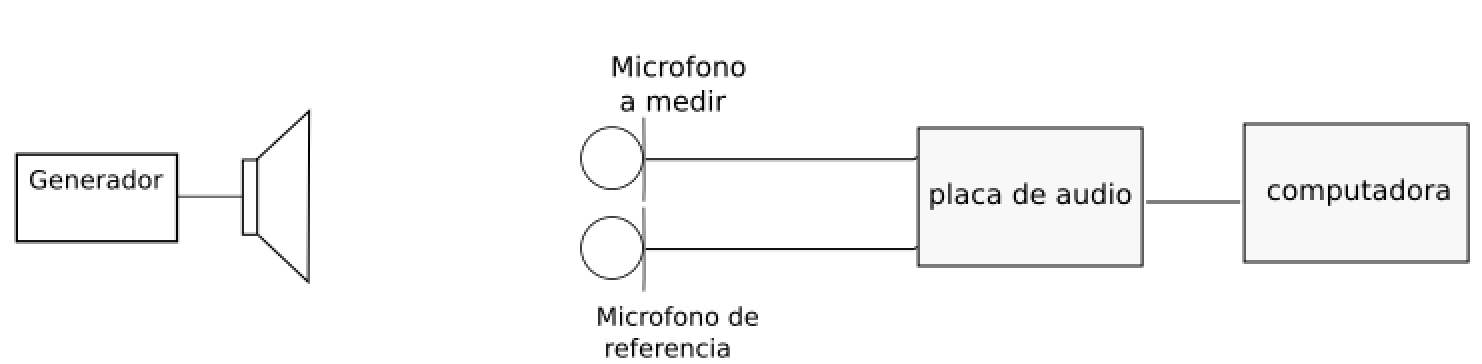
\includegraphics[width=\linewidth]{blockdiag2}
 \captionof{figure}{Arreglo instrumental del método moderno}
 \label{fig:bloque_moderno}
\end{figurehere}

Ambos micrófonos son expuestos a ruido rosa y las señales captadas por ambos
es procesada por el Software. Este ultimo compara ambas señales y bajo la
suposición que micrófono de referencia Earthworks M50 es un micrófono con
respuesta en frecuencia plana, permite obtener la respuesta en frecuencia del
micrófono a medir.

Los micrófonos medidos son : Shure SM57, Rodes NT2000, Earthworks M50 y
Beyerdynamic MM1. El Earthworks M50 y el Beyerdynamic MM1 fueron medidos en eje
y a $90^\circ$.

\section{Resultados}
En la siguiente seccion exponemos los resultados de las mediciones realizadas:
\subsection{Método clásico}

El calibrador del sonometro establece una corrección de 0.02 dB. En un intervalo
de 10 segundos, dicho sonometro indica un nivel de ruido equivalente de 75,3 dBz
. Considerando que $S_0$= $34$ mV/Pa , la sensibilidad del Shure SM57 medida es de
$1$ mV/Pa.

La tabla \ref{tab:frespsm57} presenta los resultados de la medición de respuesta en
frecuencia del micrófono Shure SM57. La tercer columna presenta los valores en dB
referidos a 1kHz.

\begin{tablehere}
\begin{center}
\begin{tabular}{|c|c|c|c|c|}
\hline
Frecuencia & Sensibilidad [mV] & Sensibilidad [dB] \\
\hline
100 Hz & 690    & -1,8 \\
500 Hz & 580    & -3,3 \\
1  kHz & 850    & 0    \\
10 kHz & 1150   & 2,6  \\
\hline
\end{tabular}
\caption{Valores obtenidos en la medición de respuesta en frecuencia del
Shure SM57}
\label{tab:frespsm57}
\end{center}
\end{tablehere}

La figura \ref{fig:aproxfrespsm57} es una representación gráfica de la información
presentada en la tabla \ref{tab:frespsm57}. Dicha figura puede considerarse una
aproximación sencilla de la respuesta en frecuencia del Shure SM57.

\begin{figurehere}
 \centering
 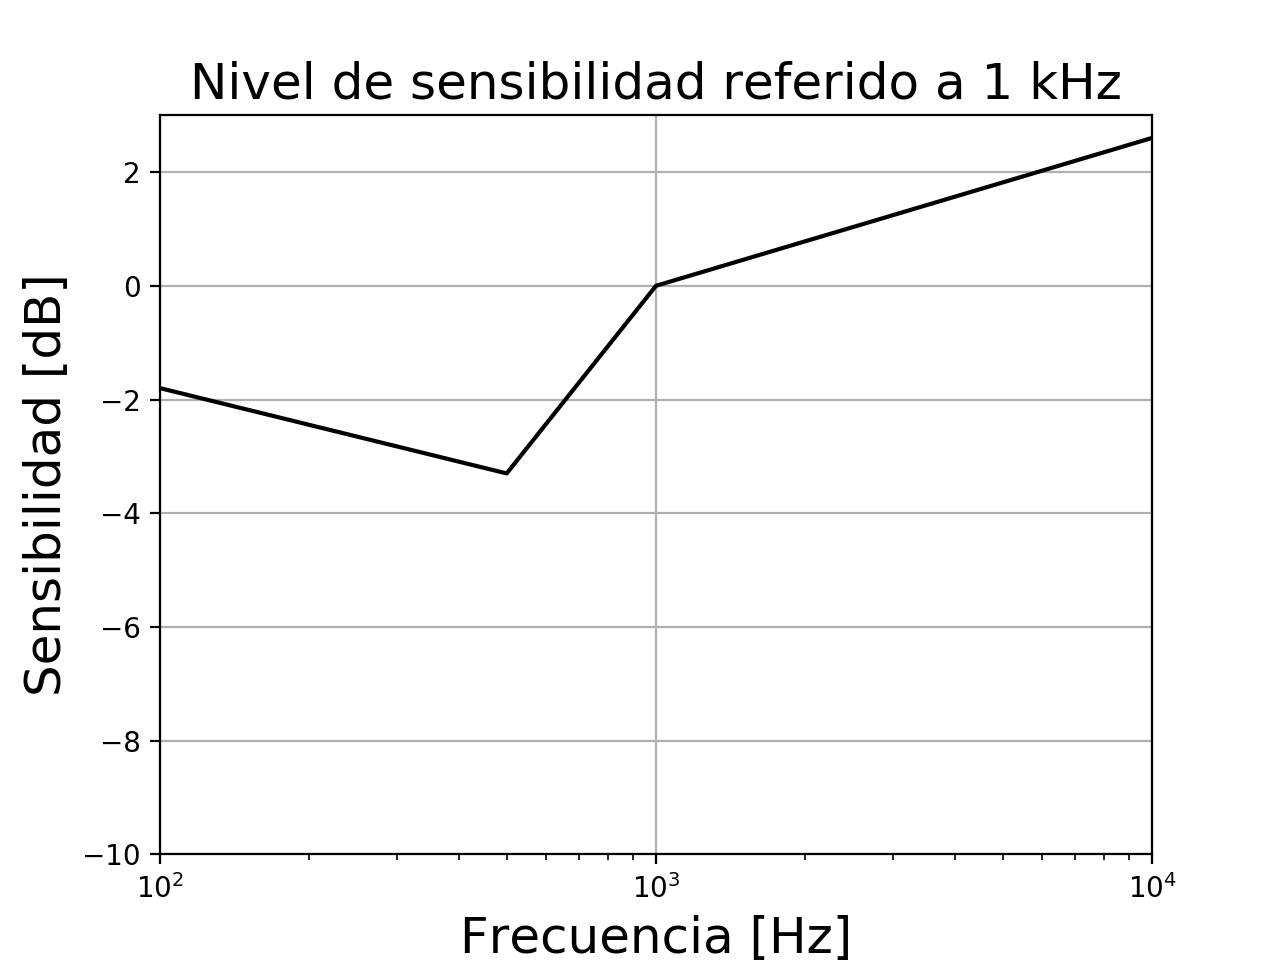
\includegraphics[width=\linewidth]{frespsm57}
 \captionof{figure}{ Aproximación de la respuesta en frecuencia del SM57}
 \label{fig:aproxfrespsm57}
\end{figurehere}


\subsection{Método moderno}
Las curvas de respuesta en frecuencia son exportados desde Smaart y graficados
mediante el uso de la libreria \textit{Matplotlib}.
El script utilizado para dicha tarea se encuentra en el Anexo A.
Las figuras \ref{fig:frespsm57} a \ref{fig:frespsm50} representan la respuesta
en frecuencia de los micrófonos medidos en este trabajo.

\begin{figurehere}
 \centering
 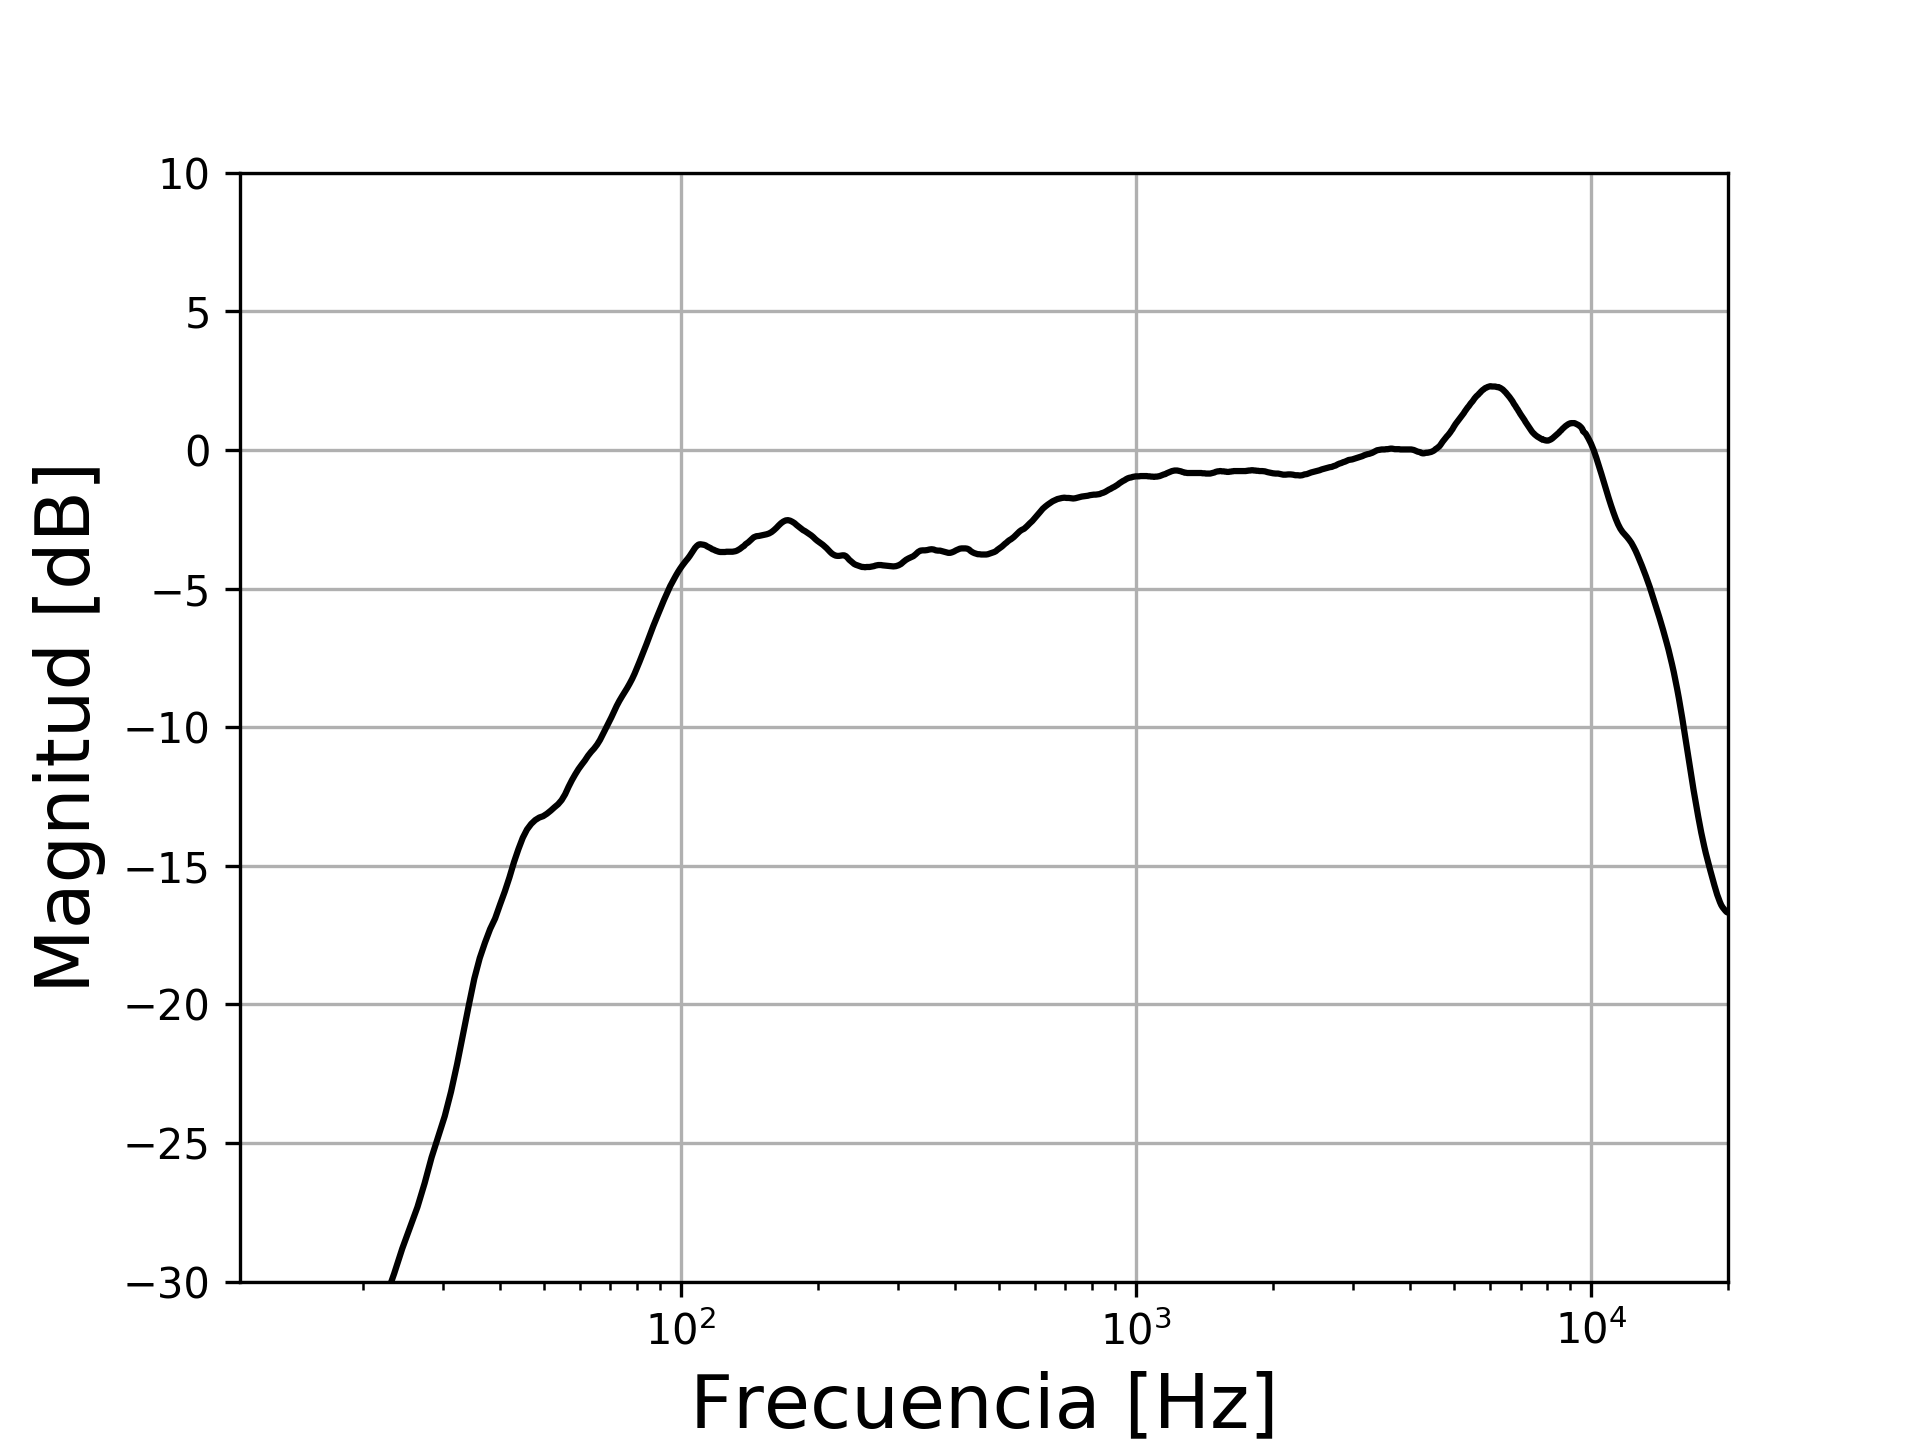
\includegraphics[width=\linewidth]{fresponse SHURE SM57}
 \captionof{figure}{Respuesta en frecuencia del SM57 obtenida}
 \label{fig:frespsm57}
\end{figurehere}

\begin{figurehere}
 \centering
 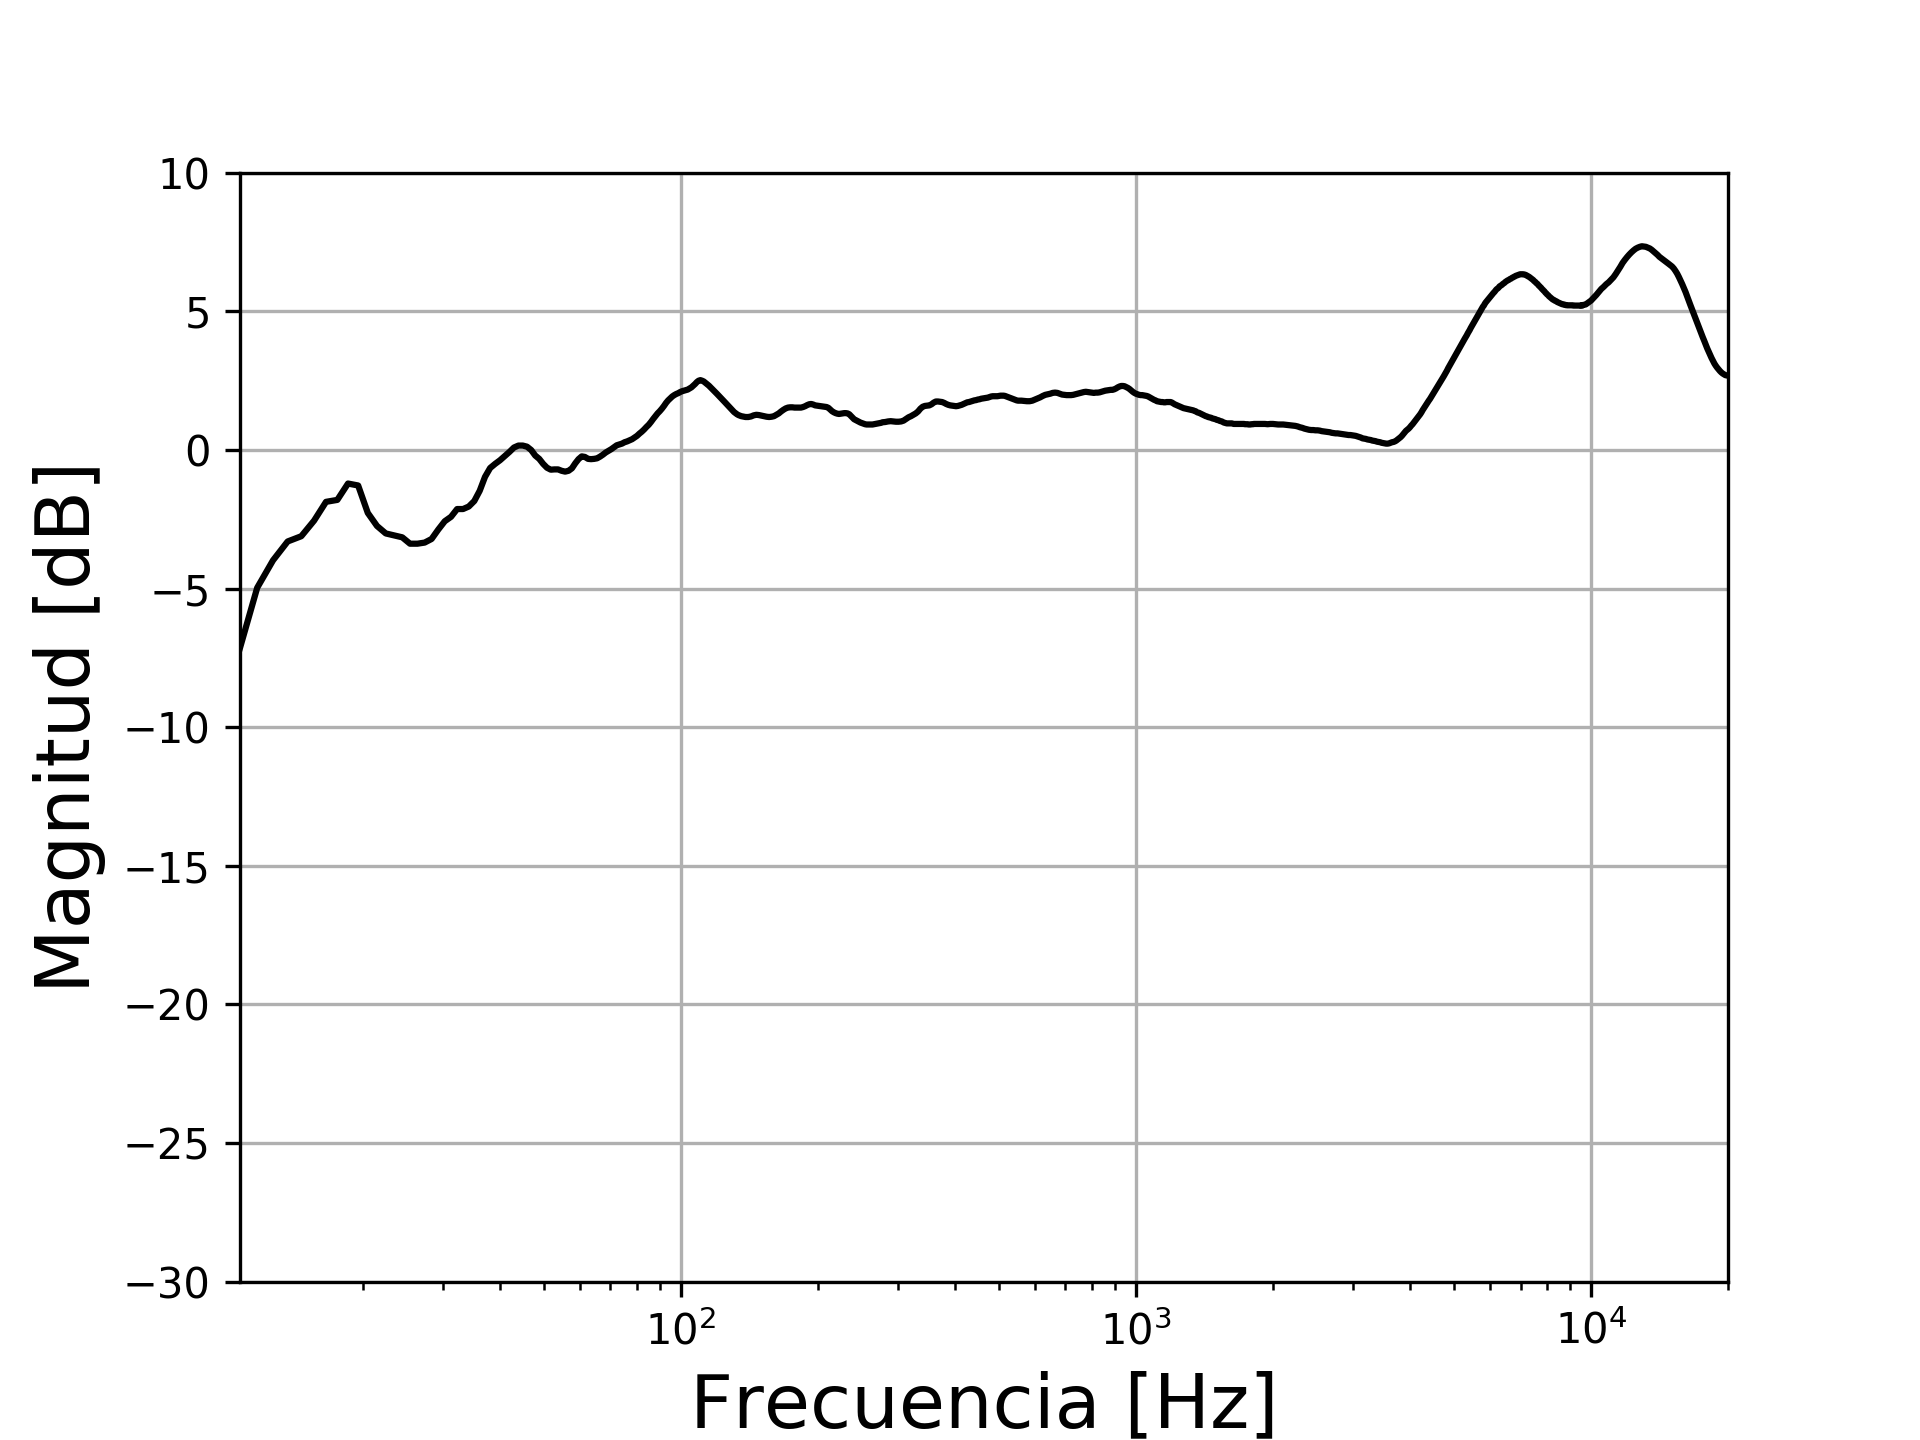
\includegraphics[width=\linewidth]{fresponse RODE NT2000}
 \captionof{figure}{Respuesta en frecuencia del Rodes NT2000 obtenida}
 \label{fig:frespsnt2000}
\end{figurehere}

El micrófono Beyerdynamic MM1 fue medido en eje y a $90^\circ$. En el caso de
la figura \ref{fig:frespmm1}, la linea sólida corresponde a la medición en eje y
la linea punteada corresponde a la medición a $90^\circ$.

\begin{figurehere}
 \centering
 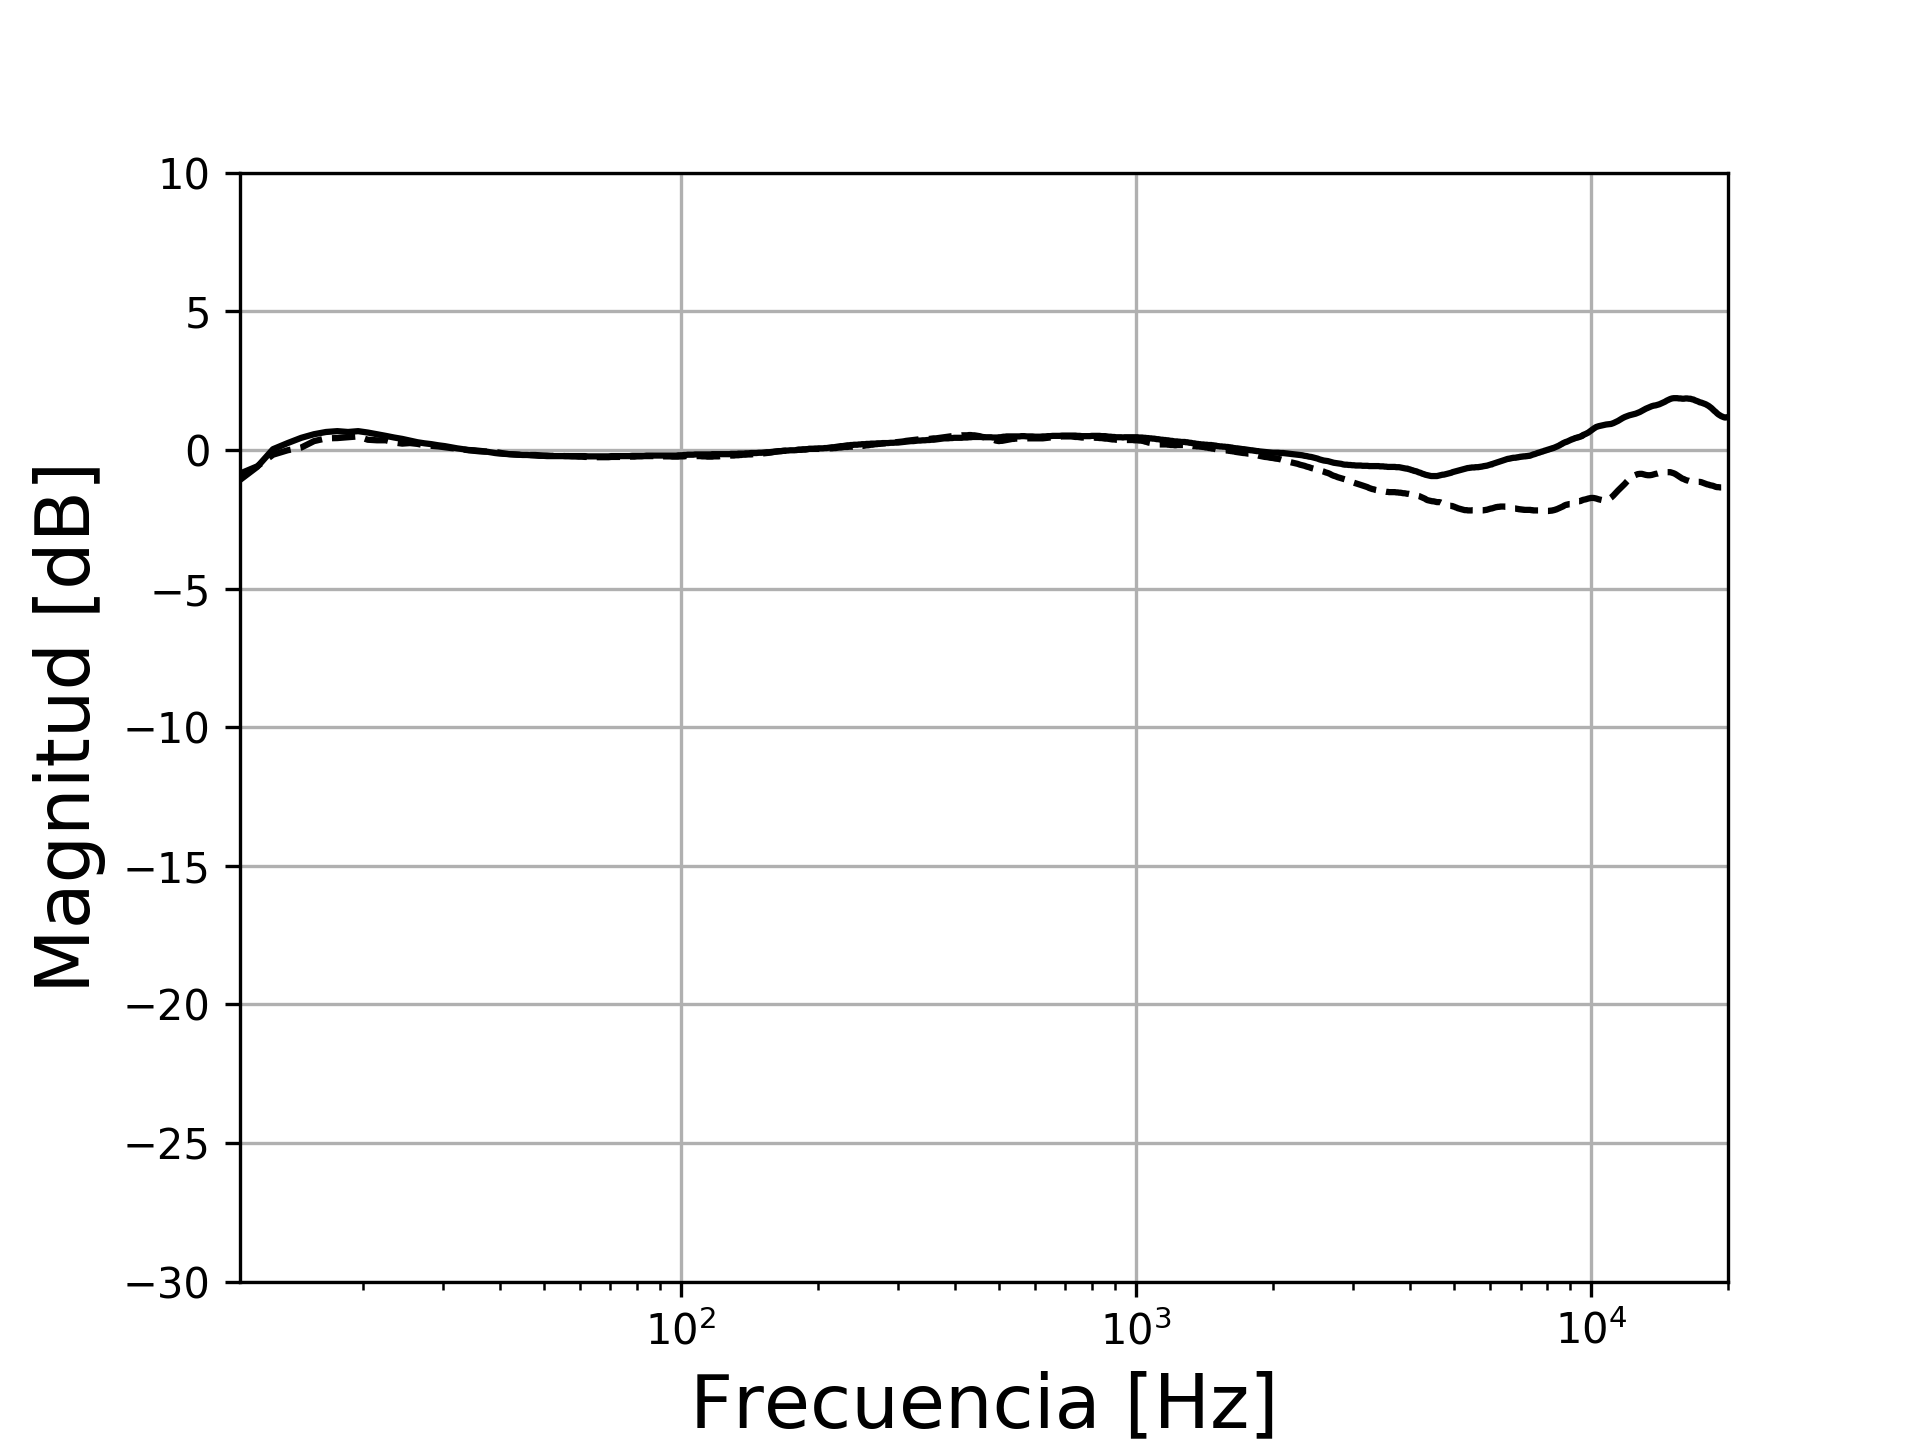
\includegraphics[width=\linewidth]{BEYERDYNAMIC MM1}
 \captionof{figure}{Respuesta en frecuencia del Beyerdynamic MM1 obtenida}
 \label{fig:frespmm1}
\end{figurehere}

El micrófono Earthworks M50 también fue medido en eje y a $90^\circ$. En el caso de
la figura \ref{fig:frespsm50}, la linea punteada corresponde a la medición en eje y
la linea solida corresponde a la medición a $90^\circ$.

\begin{figurehere}
 \centering
 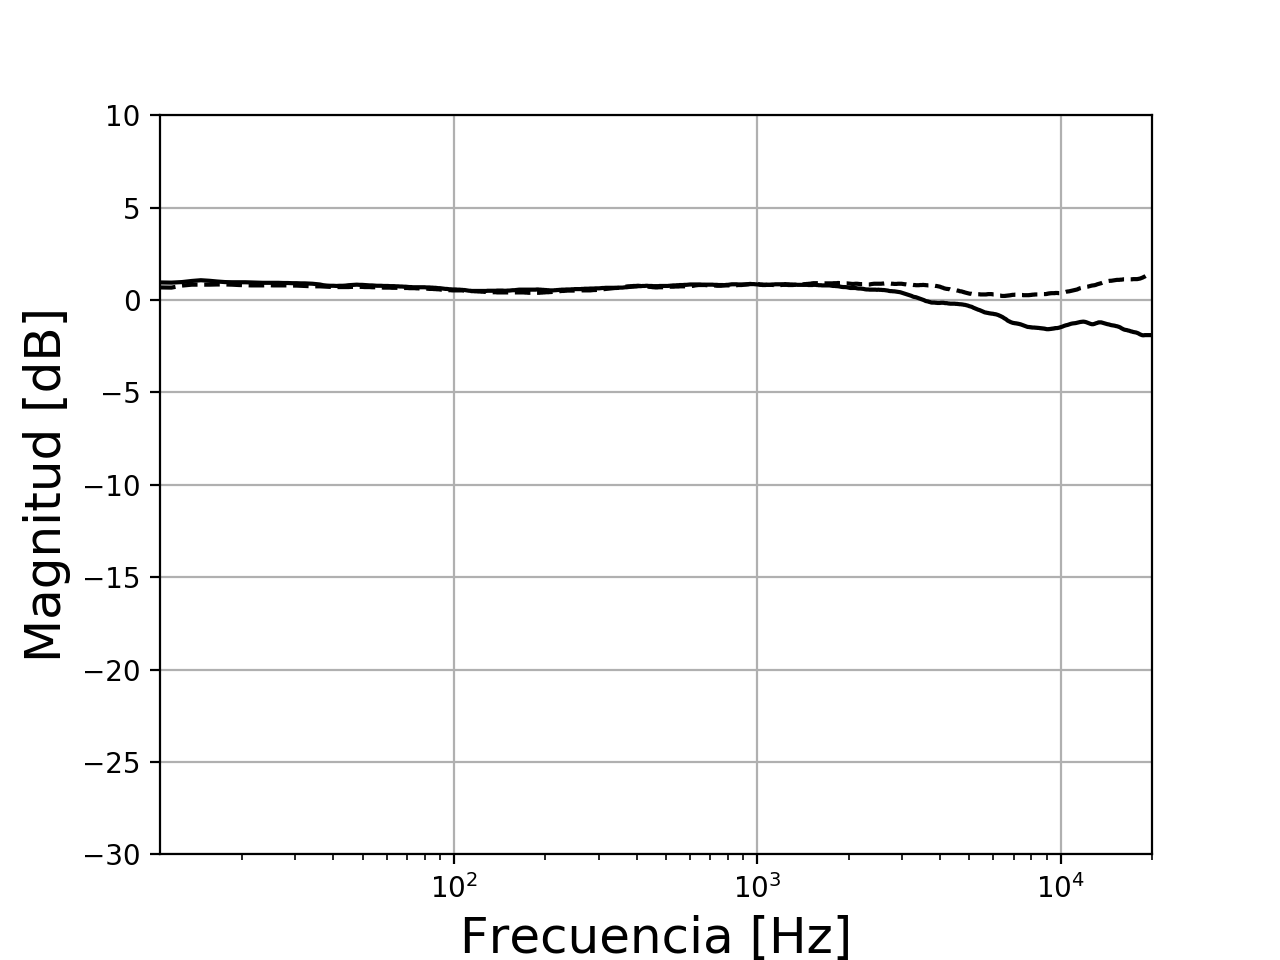
\includegraphics[width=\linewidth]{EARTHWORKS M50x2}
 \captionof{figure}{Respuesta en frecuencia del Earthworks M50 obtenida}
 \label{fig:frespsm50}
\end{figurehere}

\section{Análisis de resultados}
% Shure analog
% diferencias en la sensibilidad medida y la del datasheet
El valor de sensibilidad del SM57 medido difiere 0,6 mV respecto del valor
especificado por el fabricante. Esto es aceptable, debido al error introducido
por los dispositivos de medición. Este trabajo fundamenta la hipótesis de que
la sensibilidad del Shure SM57 es mucho mas baja que la del Earthworks M50.
Esto se debe a varios factores, pero principalmente se debe al tipo de
transducción que utiliza cada micrófono. Podemos atribuir esta diferencia a los
posibles errores de medición no contemplados, pero también se debe considerar
el posible impacto de la dispersión de fabricación.

La figura \ref{fig:aproxfrespsm57} esta basada en la información de la tabla
\ref{tab:frespsm57}. Para medir respuesta en frecuencia con cierta precisión,
el método clásico resulta muy laborioso. Debido a las limitaciones del método
clásico, solamente se tomaron  valores para 4 frecuencias diferentes. En cambio
mediante el método moderno se tomaron valores para mas de 800 frecuencias. Por
lo tanto, no podemos juzgar el comportamiento del Shure SM57 en base a la
información provista por la tabla \ref{tab:frespsm57} y la figura \ref{fig:aproxfrespsm57}.

Si consideramos la respuesta en frecuencia del Shure SM57 obtenida
mediante el método moderno, podemos comparar la figura \ref{fig:frespsm57} con la
propuesta por el fabricante \cite{shure57}. En dicha comparación se observan
discrepancias en altas frecuencias. Esto probablemente se deba al hecho que en
altas frecuencias, la longitud de onda es comparable a la distancia entre las
cápsulas del micrófono de referencia y el micrófono a medir. Bajo estas condiciones
la hipótesis de que ambas cápsulas están expuestas al mismo campo acústico se ve
debilitada.

Por otro lado, tal como era de esperar, se verifica que la sensibilidad del
Earthworks M50 es mayor que la del Shure SM57. En términos generales, podemos
afirmar que el comportamiento de el Shure SM57 y el Rode NT2000 coinciden con
las respectivas descripciones del comportamiento de un micrófono dinámico y uno
de condensador presentadas por Beranek en \cite{Beranek2012}

Al observar las figuras \ref{fig:frespsm50} y \ref{fig:frespmm1} se puede
confirmar que en bajas y medias frecuencias, ambos micrófonos exhiben un
comportamiento omnidireccional. Sin embargo, se puede observar que para alta
frecuencia, ambos micrófonos no presentan dicho comportamiento omnidireccional.

\section{Conclusiones}
% NO PUEDE FALTAR MI TP NO PUEDE FALTAR MI TP
% NO PUEDE FALTAR MI TP NO PUEDE FALTAR MI TP
El método moderno presentado en este trabajo resulta mas ágil que el método
clásico y parece otorgar resultados aceptables en cuanto a las mediciones
de respuesta en frecuencia.
Por otro lado, dicho método resulta mas fácil de reproducir debido a que requiere
de un instrumental mas sencillo que el método clásico.
Las discrepancias entre los valores medidos y los valores propuestos por los
respectivos fabricantes se atribuye tanto a la dispersión de fabricaron como
al error de medición. Dicho error es una suma de sucesivos factores de
incertidumbre dados por las condiciones ambientales y los dispositivos de
medición, particularmente de las alinealidades introducidas por el parlante,
utilizado como fuente de tonos puros.

\printbibliography

\end{multicols}

\newpage
\appendix
\section{Script en Python}
\begin{verbatim}
  import matplotlib.pyplot as plt
  import numpy as np
  def xy_a_txt(carpeta,nombre,col1,col2,xscale,xmin,xmax,ymin,ymax,size,xlabel,ylabel):
      filename = carpeta+nombre+'.txt'
      name=carpeta+'fresponse '+ nombre
      data = open(filename) # open file with names in
      rbfile = data.readline()                # read data file name
      x = np.genfromtxt(filename,skip_header=2,usecols=(col1))
      y = np.genfromtxt(filename,skip_header=2,usecols=(col2))
      plt.plot(x,y,color='black')
      plt.xscale(xscale)
      plt.axis([xmin,xmax,ymin,ymax])
      plt.xlabel(xlabel, fontsize=size)
      plt.ylabel(ylabel, fontsize=size)
      plt.grid(True)
      plt.savefig(name,dpi=300)

\end{verbatim}
\end{document}
